\documentclass[11pt]{beamer}
\usetheme{Warsaw}
\usepackage[utf8]{inputenc}
\usepackage[spanish]{babel}
\usepackage{amsmath,amsthm,amssymb} %modos matemáticos y  simbolos
\usepackage{mathrsfs}
\usepackage{latexsym,amsfonts} %simbolos matematicos
\usepackage{graphicx}
\usepackage{physics} %Simbolos fisicos
\usepackage{array} %mejores formatos de tabla
\usepackage{tabulary}
\usepackage{multirow} %ocupar varias filas en una tabla
\usepackage{fancybox} %recuadros talegas
\usepackage{float} %ubicar graficas
\usepackage{color}
\usepackage{comment}
\usepackage{stackrel}
\usepackage{calligra}
\usepackage{lipsum} % texto de relleno
\usepackage{cite}
\author{Diego Sarceño}
\title{Métodos Matriciales en Óptica Paraxial}
%\setbeamercovered{transparent} 
%\setbeamertemplate{navigation symbols}{} 
%\logo{} 
%\institute{} 
\date{\today} 
%\subject{} 
\begin{document}

\begin{frame}
\titlepage
\end{frame}

%\begin{frame}
%\tableofcontents
%\end{frame}

\frame{
	\frametitle{Enunciado del Problema}
	Se tiene la parte final de una varilla larga de plástico de ínice de refracción $n_2 = 1.56$ pulida a una superficie esférica convexa de radio $r = 2.8cm$. Un objeto de $2cm$ de alto, está localizado en el aire y en el eje a una distancia de $15cm$ del vértice. (vease la figura \ref{prob1}) Encuentre la posición y el tamaño de la imagen dentro de la varilla.
}


\frame{
	\frametitle{Figura}
	\begin{figure}
		\centering
		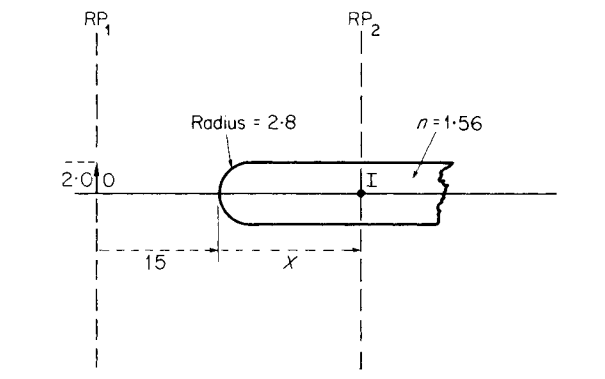
\includegraphics[scale=0.5]{img/problema1.png}
		\caption{Varilla de plástico y objeto.}
		\label{prob1}
	\end{figure}
}


\frame{
	\frametitle{Solución}
	Encontramos las matrices para cada una de las partes involucradas en el sistema (sustituyendo los valores correspondientes):
	\begin{description}
		\item[Matriz de Refracción: ] Se tiene
			$$ \mathscr{R} = \mqty(1 & 0 \\ -\frac{(n_2 - n_1)}{r} & 1) = \mqty(1 & 0 \\ -0.2 & 1). $$
		\item[Imagen a la Superficie: ] 
			$$ \mathscr{F} = \mqty(1 & \frac{x}{n} \\ 0 & 1). $$
		\item[De la Superficie al Objeto: ] 
			$$ \mathscr{O} = \mqty(1 & 15 \\ 0 & 1). $$
	\end{description}
}


\frame{
	\frametitle{Solución}
	Entonces, la cadena de productos matriciales está dada como
		$$ M = \mathscr{F} \mathscr{R} \mathscr{O} .$$
	Sustituyendo valores y operando en mathematica
		$$ M = \left(
\begin{array}{cc}
 1\, -0.128205 x & 15\, -1.28205 x \\
 -0.2 & -2 \\
\end{array}
\right) . $$
Dada la relación Objeto$-$Imagen, se tiene que el elemento $B$ debe ser nulo y que $A = \flatfrac{1}{D}$, para la matriz
	$$ \mqty(A & B \\ C & D); $$
por lo que, el valor de $x$ esta dado como
}


\frame{
	\frametitle{Solución}
	$$ 15 - 1.28205x = 0 \qquad \rightarrow \qquad \boxed{x = 11.7cm}. $$
	Para el tamaño de la imagen se utiliza la magnificación, es decir, $A = \flatfrac{1}{D} = -0.5$, por lo que el tamaño de la imagen es $A*2cm = \boxed{1cm}$ y esta invertida.
}


\frame{
	\centering
	\vspace{1cm}
	GRACIAS POR SU ATENCIÓN $<3$
}














\end{document}